\chapter{Closed-Loop Subspace Identification of a Quadrotor}\label{results}

Results section should follow the methods section

Make sure you interpret the results too, don't just present them!

\section{Identified Model Overview}
Through application of the Innovation Estimation Method as outlined in Chapter \ref{approach}, we developed an 8th order LTI model of a quadrotor from experimentally gathered closed-loop input-output data. In its state space form, the model is given by
\begin{subequations}\label{eq:2_lti}
\begin{equation*}x(k+1) = Ax(k) + Bu(k)\end{equation*}
\begin{equation*}y(k) = Cx(k) + Du(k)\end{equation*}
\end{subequations}
with
\footnotesize % DECREASE FONT SIZE
\begin{equation*}
A = \begin{bmatrix}
0.8119&0.1408&-0.4270&0.3362&0.0193&-0.0159&0.0471&0.0798\\
0.0168&0.2216&0.6307&0.6795&-0.0599&-0.1555&-0.1142&-0.0120\\
0.0366&0.7002&0.1693&-0.2331&0.5229&0.1084&0.3362&0.0415\\
-0.1893&-0.1149&-0.2148&0.1636&0.6510&0.0198&-0.4611&-0.1186\\
-0.0453&0.0245&0.0303&0.1571&-0.1532&0.8764&0.0014&-0.1361\\
0.0630&-0.1064&0.1144&0.0451&-0.0730&-0.1346&0.2610&-0.5882\\
0.0218&-0.1402&-0.0459&0.1871&0.2132&0.2603&0.0161&-0.2477\\
-0.0439&0.0445&0.0417&0.0807&-0.0606&0.1664&-0.2713&0.5972
\end{bmatrix};
\end{equation*}
\begin{equation*}
B = \begin{bmatrix}
   -0.0025&0.0017&-0.0017&0.0019\\
   -0.0007&-0.0011&0.0028&0.0008\\
   -0.0043&-0.0005&0.0047&-0.0013\\
   -0.0029&0.0027&-0.0017&-0.0026\\
    0.0015&-0.0003&0.0021&-0.0001\\
   -0.0003&-0.0004&0.0002&0.0009\\
    0.0007&0.0020&-0.0003&0.0005\\
    0.0007&0.0006&0.0028&-0.0023
\end{bmatrix};
\end{equation*}   
\begin{equation*}
C = \begin{bmatrix}
-0.0001&0.0001&-0.0000&0.0002&-0.0001&0.0000&0.0000&-0.0000\\
0.0002&-0.0000&0.0001&-0.0002&0.0003&-0.0000&-0.0001&0.0001\\
-0.0000&-0.0000&-0.0002&0.0008&0.0003&-0.0003&0.0008&0.0003\\
-0.3177&-0.2832&-0.2047&0.4147&0.2051&-0.0510&0.6507&0.3091\\
-0.4332&0.5501&-0.5182&0.2348&-0.3507&-0.1015&-0.0689&-0.1618\\
-0.0043&-0.0518&-0.0137&0.0233&-0.0054&0.0017&-0.0157&0.0218
\end{bmatrix};
\end{equation*} 
\begin{equation*}
D = \begin{bmatrix}
0&0&0&0\\
0&0&0&0\\
0&0&0&0\\
0&0&0&0\\
0&0&0&0\\
0&0&0&0
\end{bmatrix}
\end{equation*}
\normalsize % INCREASE FONT SIZE
The resulting model takes four motor inputs and produces accelerations for three axes ($\ddot x, \ddot y, \ddot z$) and angular rates about the three body axes ($p, q, r$). The model order was selected by partitioning the SVD of the extended observability matrix into two portions: one representing the identified system's dynamics and the remaining portion representing noise. From Figure \ref{fig:5_singular_values}, a model order between 1 and 13 appears to capture the significant system responses. Evaluating model orders in this range revealed that an 8th order model provided the best overall system performance, which is the resulting model presented here. 
\begin{figure}[htb!]\label{fig:5_singular_values}
	\centering
	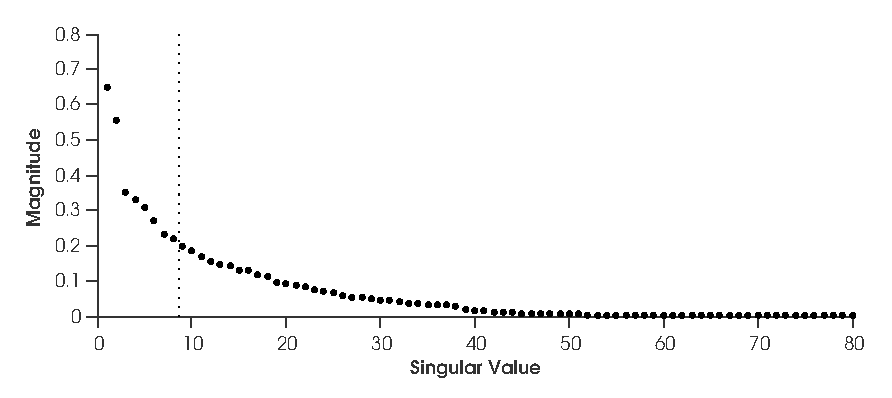
\includegraphics{../fig/singular_values_parsim.eps}
	\caption{A plot of the singular values of the extended observability matrix, used to determine the model order. The vertical dotted line shows the partitioning location between system response and noise in the final 8th order model.}
\end{figure}


\begin{figure}[htb!]
	\centering
	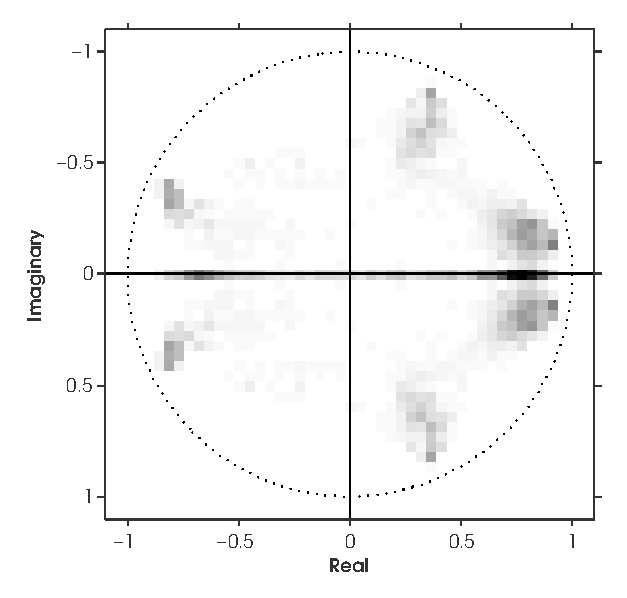
\includegraphics{../fig/poles_parsim_all.eps}
	\caption{Quadrotor test flight profile showing the portion of the test flight data used for system identification.}
\end{figure}

\begin{figure}[htb!]
	\centering
	\includegraphics{../fig/poles_parsim.eps}
	\caption{Quadrotor test flight profile showing the portion of the test flight data used for system identification.}
\end{figure}


Stimulating the system with a step response provides insight into the model performance (Figure \ref{fig:5_step}).
\begin{figure}[htb!]\label{fig:5_step}
	\centering
	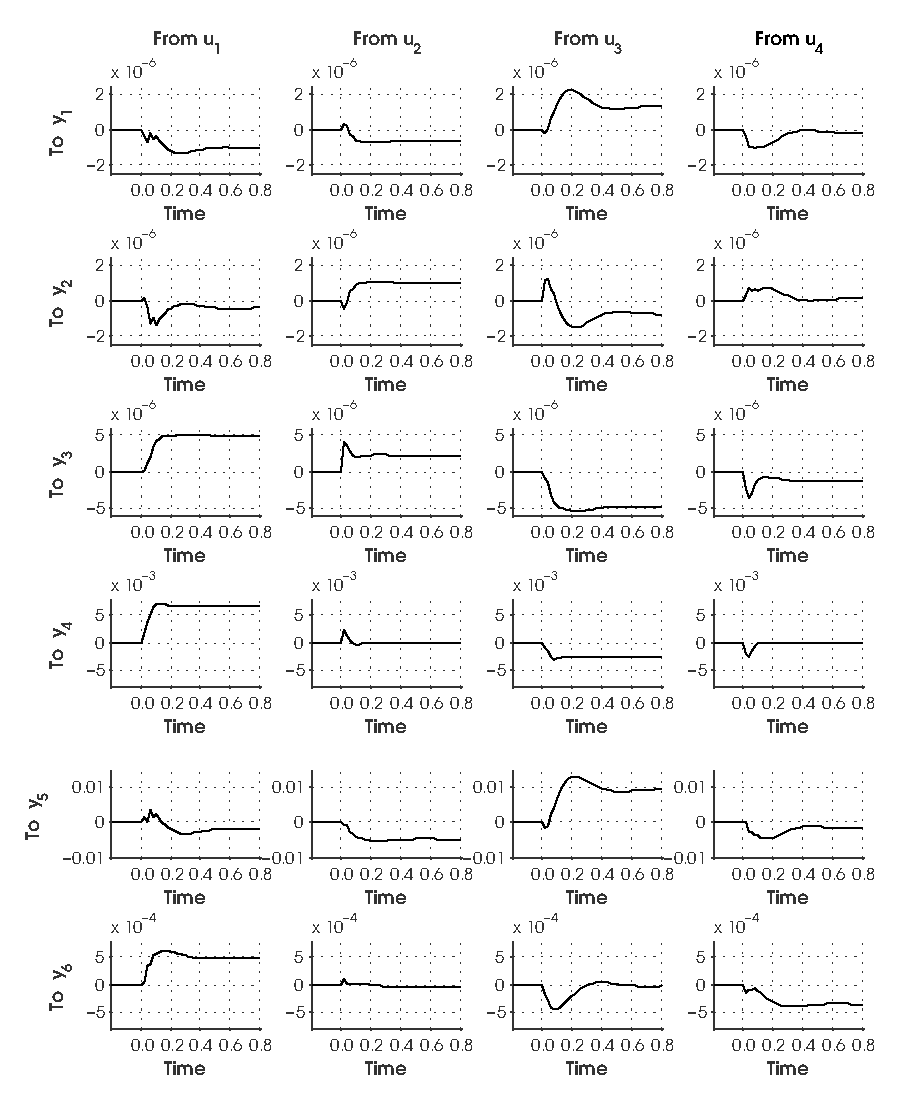
\includegraphics{../fig/step_resp_parsim.eps}
	\caption{Step response of the 8th order system model.}
\end{figure}



\section{Time Domain Model Validation}
Leong\_2008 p. 63 for validation



\section{Comparing Performance of PO-MOESP and IEM Algorithms on Closed-Loop Data}
